% Author: Giulio Stramondo, Mail: giuliostramondo[at]gmail.com
\documentclass{standalone}
\usepackage{tikz}
\usetikzlibrary{shapes.gates.logic.US,shapes.geometric,trees,positioning,arrows,calc}
\begin{document}
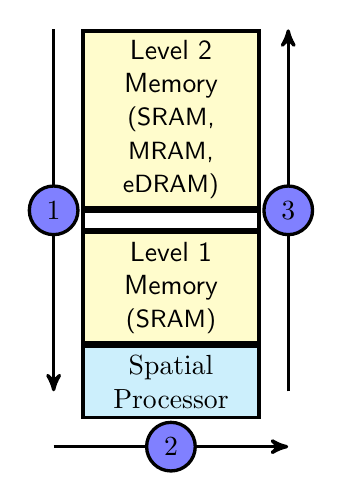
\begin{tikzpicture}[
    bus/.style={rectangle,thick,draw,anchor=north,
		minimum width=1.5cm,minimum height = 0.5mm},
    archb/.style={rectangle,thick,draw,fill=blue!60,anchor=north,
		minimum width=0.2cm},
    archm/.style={rectangle,thick,draw,fill=magenta!60,anchor=north,
		minimum width=0.2cm},
    select/.style={circle,thick,draw,anchor=north,
		minimum width=0.4cm},
% Event style
    event/.style={rectangle,very thick,draw,fill=yellow!20,text width=2cm,
		text centered,font=\sffamily,anchor=north},
%  For compatability with PGF CVS add the absolute option:
   absolute
    ]
   \begin{scope}[xshift=-7.5cm,yshift=-5cm,very thick,
		node distance=1.6cm,on grid,>=stealth',
		block/.style={rectangle,draw,fill=cyan!20,text width=2cm,text centered}]
\node [event] (memoryl2) {Level 2\\Memory\\ \small (SRAM, MRAM, eDRAM)};
\node [event,fill=white,below=of memoryl2.south,below=0pt] (separation) {};
\node [event,below=of separation.south,below=0pt] (memoryl1) {Level 1\\Memory\\ \small (SRAM)};
\node [block, below=of memoryl1.south,below=0pt] (processor) {Spatial\\Processor};

\draw [->] ([xshift=-10pt]memoryl2.north west) -- ([xshift=-10pt,yshift=10pt] processor.south west)
node [circle,draw,fill=blue!50] [pos=1/2] {1};
\draw [->] ([xshift=-10pt,yshift=-10pt] processor.south west) --  ([xshift=10pt,yshift=-10pt] processor.south east)
node [circle,draw,fill=blue!50] [pos=1/2]{2} ;
\draw [->] ([xshift=10pt,yshift=10pt] processor.south east) --  ([xshift=10pt]memoryl2.north east)
node [circle,draw,fill=blue!50] [pos=1/2]{3} ;
\end{scope}
\end{tikzpicture}
\end{document}
